%%%%%%%%%%%%%%%%%%%%%%%%%%%%%%%%%%%%%%%%%%%
%+ Chuong 1. Co so ly thuyet ma.
%+ Revised: 03-05-2008
%+ Last revised: 10-05-2008
%%%%%%%%%%%%%%%%%%%%%%%%%%%%%%%%%%%%%%%%%%%
\setcounter{chapter}{0}
\chapter{CƠ SỞ LÝ THUYẾT MÃ}

Trong chương này, chỉ những khái niệm cơ bản liên quan được sử dụng trong luận án mới được đề cập. Nội dung kiến thức về đại số, ngôn ngữ và mã của các từ hữu hạn trình bày trong các mục,
từ Mục \hyperlink{page.6}{\textcolor{blue}{1.1}} đến Mục \hyperlink{page.16}{\textcolor{blue}{1.4}}, được tham khảo và trích dẫn từ các tài liệu [\textcolor{red}{4; 5; 6; 7; 9; 13; 16; 18; 21; 27; 28}].. Bên cạnh đó, luân án còn giới thiệu một số lớp mã dựa trên các hình thức tích mới, hiệu quả của các lớp mã này trong các chương tiếp theo. Nội dung kiến thức về mã luân phiên và mã của các từ định biên trong trình bày trong Mục \textcolor{blue}{1.5} là một hướng nghiên cứu mới trong lý thuyết mã, được đề xuất gần đây trong các công trình [\textcolor{red}{14; 15; 23; 32; 33; 34; 35}]. Kiến thức về ngôn ngữ và mã của các từ vô hạn xem như một sự mở rộng các khái niệm trong lý thuyết mã truyền thống trường hợp vô hạn được tổng hợp từ các tài liệu [\textcolor{red}{3; 10; 11; 13; 19; 20; 24; 29; 31}], là nội dung của mục \textcolor{blue}{1.6}.
Trong luận án tập các số tự nhiên được ký hiệu là $\mathbb{N}$. Lực lượng của 1 tập hợp $X$ được ký hiện là Card($X$). Các bảng chữ đều được giả thiết là hữu hạn nếu không nói gì khác.
%*************************************************************************
%+ 1.1. Nua nhom va vi nhom
%************************************************************************
\section{Nửa nhóm và vị nhóm}

Ta nhắc lại rằng một nửa nhóm S là một tập hợp được trang bị một phép toán hai ngôi kết hợp, nếu không nói gì thêm ta sẽ ký hiệu theo lỗi nhân. Một nửa nhóm con (t.ư. nhóm con) T của S là một tập con 
của S cùng với phép toán cảm sinh là cho T trở thành nửa nhóm (t.ư. nhóm). Nửa nhóm S là một vị nhóm nếu S có đơn vị. Đơn vị của vị nhóm S là duy nhất và được ký hiệu là $1_S$.
Một vị nhóm con của vị nhóm S là một nửa nhóm con có chứa đơn vị của S.


\textit{Ví dụ 1.1.} $M = \{0,1\}$ là vị nhóm nhân với phần tử đơn vị là 1.

\textit{Ví dụ 1.2.}
    Với vị nhóm $M$ bất kỳ, ta trang bị cấu trúc vị nhóm cho tập tất cả các tập con $\mathcal{P}(M)$ của M bằng cách định nghĩa, với $X, Y \subset M$,
    $$
        XY = \{ xy | x \in X, y \in Y \}
    $$
    Phần tử đơn vị là $\{1\}$.
1.1 Nửa nhóm và vị nhóm
\textit{Ví dụ 1.3.} 
    Từ các vị nhóm $M, N$ ta có vị nhóm $M \times N$ là tích trực tiếp của $M$ và $N, M^{(n)}$ là tích trực tiếp của $n$ lần vị nhóm $M$.

    Cho các nửa nhóm (vị nhóm) $S$ và $T$. Ánh xạ $\varphi : S \rightarrow T$ được gọi là một {\it đồng cấu nửa nhóm} (t.ư. {\it vị nhóm}) nếu với mọi $a, b \in S$,
    $$
    \varphi(ab) = \varphi(a)\varphi(b)
    $$
    (t.ư $\varphi(ab) = \varphi(a)\varphi(b)$ và $\varphi(1_S) = 1_T$ với $1_S$ là đơn vị của $S$, $1_T$ là đơn vị của $T$).

    Đồng cấu $\varphi$ được gọi là {\it đơn cấu} (t.ư {\it toàn cấu, đẳng cấu}) nếu $\varphi$ là đơn ánh (t.ư. toàn ánh, song ánh). 
    Một đồng cấu từ vị nhóm $S$ vào chính nó thì được gọi là một {\it tự đồng cấu}.
    Một {\it tương đẳng} trên một vị nhóm $M$ là một quan hệ tương đương ${\theta}$ trên $M$ sao cho với mọi $m,m' \in M, u,v \in M$
    $$
    m \equiv m'mod\theta \Rightarrow umv \equiv um'vmod\theta 
    $$
    \hspace{10mm} Nếu $\varphi : M \to N$ là một đồng cấu vị nhóm thì {\it quan hệ} ({\it hạt nhân}) $\equiv_\varphi$ trên $\theta$, cho bởi $m \equiv_\varphi m'mod\theta {\Leftrightarrow}$ $\varphi(m) = \varphi(m')$ là một tương đẳng trên $M$. Ngược lại nếu $\theta$ là một tương đẳng trên vị nhóm $M$, tập thương $M/\theta$ với phép toán $[x]_\theta[y]_\theta = [xy]_\theta$, ở đó $[x]_\theta$ kí hiệu tương đương theo $\theta$ chưa $x$, là một {\it vị nhóm thương} của $M$ với tương đẳng $\theta$ và ta có {\it đồng cấu tự nhiên} $\theta^\aleph : M \to M/\theta$ cho bởi $\theta^\aleph(m) = [m]_\theta$ với mọi $m \in M$.\\
    Cho $M$ là một vị nhóm. Với $x, y \in M$, ta có: 
    \center{    
        $x^{-1}y = \{z \in M | x.z = y\} $ và $ xy^{-1} = \{z \in M | x= z.y \}.$
    }\\
    \begin{flushleft}
    \hspace{10mm} Với $S, T \subseteq M$, ta định nghĩa các phép cắt trái, phải của $S$ bởi $T$
    \end{flushleft}
    $
    T^{-1}S = \{u \in M \exists \in T : t.u \in S \}$ và $ST^{-1} = \{ u \in M \exists \in T : u.t \in S \}
    $
    \begin{flushleft}
    \hspace{10mm}Ta có tính chất cơ bản sau
    \end{flushleft}
\begin{flushleft}
    \textbf{Tính chất 1.1}  Cho $M$ là một vị nhóm , $P,K \subseteq M, P = K^*$ và $m \in M$. Khi đó $P^{-1}(m^{-1})K = (m.P)^{-1}K$.\\
    {\it Chứng minh.} Chứng minh $P^{-1}(m^{-1})K \subseteq (m.P)^{-1}K$. Ta có\\
    \hspace{10mm} $\omega \in P^{-1}(m^{-1})K \Leftrightarrow (\exists p \in P, k \in K : \omega = p^{-1}( m^{-1}k ) \Leftrightarrow k = m.p.\omega).$ \\
    Vi vậy $\omega = (m.p^{-1}k \in (m.P)^{-1}K.$ \\
    \hspace{10mm}Chứng minh $P^{-1}(m^{-1})K \subseteq P^{-1}( m^{-1}K )$. Ta có \\
    \hspace{20mm} $\omega \in ( m.P )^{-1}K \Leftrightarrow ( \exists p \in P , k \in K : \omega = ( m.p )^{-1}k \Leftrightarrow k = m.p.\omega ).$ \\
    Vì vậy $\omega = p^{-1}( m^{-1}k ) \in P^{-1}( m^{-1}K )$
\end{flushleft}
%+ Dinh nghia 1.1.1
\begin{definition}\label{de.1.1.1} 
Giả sử $C\subseteq R^n$ là một tập hợp khác rỗng.
\begin{itemize}
\item Tập $C$ gọi là tập lồi nếu với mọi $x,y\in C$ và mọi  $\lambda\in [0,1]$ ta có
$$\lambda x+(1-\lambda)y\in C$$

\item Giả sử $x^1,\dots, x^k$ là $k$ điểm của $C$ khi đó 
\begin{equation}\label{eq.1.1.1}
x  = \sum\limits_{i=1}^k\lambda_kx^k,\quad\text{với}\quad \lambda_k\geq 0,\sum\limits_{i=1}^k\lambda_k=1,\forall k =1,\ldots,k
\end{equation}
gọi là một tổ hợp lồi của hệ vector  $\{x^1,\ldots, x^k\}$.
\end{itemize}
\end{definition}
Cho $M\subseteq R^n$, ta nói bao lồi của một tập hợp $M$ là giao của tất cả các tập lồi chứa $M$, được kí hiệu là $\text{conv}(M)$. Rõ ràng bao lồi của $M$ là tập lồi nhỏ nhất chứa $M$. Một tập $C$ là lồi khi và chỉ khi nó chứa mọi tổ hợp lồi hữu hạn các điểm của $C$.

Một trong những tập lồi quan trọng (trong giải tích lồi, tối ưu (đặc biệt là quy hoạch tuyến tính)) là tập lồi đa diện. 
Tập lồi $P$ được gọi là tập lồi đa diện nếu $C$ có dạng
\begin{equation}\label{eq.1.1.2}
P := \{x\in R^n\; |\; Ax \leq b\}
\end{equation}
trong đó $A=(a_{ij})_{m\times n}, b\in R^m$. Hay nói cách khác, $P$ là giao của hữu hạn các nửa không gian đóng.
Trường hợp đặc biệt của tập lồi đa diện là đa diện chính tắc có dạng như sau:
\begin{equation}\label{eq.1.1.3}
P_0 := \set{x\in R^n\; |\; Ax = b, x\geq 0 }
\end{equation}
trong đó ma trận $A\in\R^{m\times n}, b\in\R^m$ và giả thiết $A$ có hạng đủ (tức là $\text{rank}A = m\leq n$).

%+ Dinh nghia 1.1.2.
\begin{definition}\label{de.1.1.2}\
\begin{itemize}
\item Tập $C$ được gọi là một nón nếu với mọi $x\in C$ và mọi $\lambda\geq 0$ ta có $\lambda x\in C$.
\item Tập $C$ được gọi là nón lồi nếu $C$ vừa là nón vừa là tập lồi.
\end{itemize}
\end{definition}
Bao nón lồi của tập $M$ là giao của tất cả các nón lồi chứa $M$, ký hiệu là $\text{conv}(M)$ và nó cũng là tập nón lồi nhỏ nhất chứa $C$. Nói $C$ gọi là nón lồi đa diện nếu $C$ vừa là nón vừa là tập lồi đa diện. Mỗi nón $C$ có một điểm $x=0$ gọi là gốc (mũi) của nón $C$. Tập $r:=\set{x\in C: x=x^0+\lambda d}$ gọi là một tia xuất phát từ $x^0$ theo hướng $d\neq 0$. Một nón $C$ sẽ chứa các tia xuất phát từ $x^0=0$.\\
Cho một tập lồi đa diện $P=\set{x\in\R^n\;:\; Ax=b}$ với $\text{rank} A=m\leq n$. Khi đó tập $K:=\set{d\;|\; Ad \geq 0}$ là một nón lồi đa diện, gọi là nón lồi sinh ra bởi các hướng cực biên của $P$ (như định nghĩa dưới đây). 

%+ Dinh nghia 1.1.2.
\begin{definition}\label{de.1.1.2}\
\begin{itemize}
\item Điểm $x^0$ là điểm cực biên (hai đỉnh) của tập lồi đa diện $P$ nếu nó không là điểm trong của bất kỳ đoạn nào nối hai điểm khác nhau của $P$, tức là $\nexists x', x'' \in P$ và $x' \neq x''$ sao cho 
$$
x^0 = \alpha x'+(1-\alpha)x''
$$
với $\alpha$ nào đó thuộc $(0,1)$.
\item Mỗi tập con $L$ của đa diện lồi $P$ gọi là một cạnh nếu với mọi $x,y\in P, \lambda\in (0,1)$ mà $\lambda x+(1-\lambda)y\in L$ thì $[x,y]\subseteq L$ và $L$ chứa trọn trong một đường thẳng. Một cạnh vô hạn gọi là một tia cực biên. Hướng của tia cực biên này gọi là hướng cực biên của $P$.
\end{itemize}
\end{definition}
Chú ý rằng, tập lồi đa diện đóng, bị chặn thì không có hướng cực biên. Số đỉnh và số hướng cực biên của tập lồi đa diện $P$ là hữu hạn.

%+ -------------------------------------------------------------------------------------------
%+ 1.1.2. Mot so dinh ly quan trong.
\begin{flushleft}
\subsection{Một số kết quả trong giải tích lồi}
\end{flushleft}
Phần này trình bày một số kết quả đã được đề cập trong giải tích lồi có liên quan đến khóa luận. Trước hết, cần nhắc lại một trong những định lý quan trọng là định lý biểu diễn tập lồi đa diện.
%+ Dinh ly 1.1.1. (Ve bieu dien tap loi da dien)
\begin{theorem}\label{th.1.1.1} 
Cho $P$ là tập lồi đa diện trong $\R^n$ với tập đỉnh là $V:=\set{v^i: i=1\dots,p}$ và tập các hướng cực biên là $E:=\set{d^j: j=1\dots q}$. Khi đó mọi điểm $x\in P$ đều có thể biểu diễn dưới dạng:
\begin{equation}\label{eq.1.1.2.1}
x = \sum_{i=1}^p\lambda_iv^i + \sum_{j=1}^q\gamma_jd^j,
\end{equation}
trong đó $\sum_{i=1}^p\lambda_i = 1, \lambda_i\geq 0, i=1,\dots,p$ và $\gamma_j\geq 0, j=1,\dots, q$.
\end{theorem}
Hiển nhiên nếu $P$ là đa diện lồi bị chặn thì biểu diễn chỉ còn lại
$$
x = \sum_{i=1}^p \lambda_iv^i.
$$
Một tập lồi đa diện khác rỗng, không chứa trọn một đường thẳng thì luôn có điểm cực biên và số điểm cực biên là hữu hạn. Để kiểm tra một điểm $x^0$ có là điểm cực biên của tập lồi đa diện, ta có định lý sau.

%+ Dinh ly 1.1.2. ( Xac dinh diem cuc bien (lam the nao kiem tra mot diem cua tap loi da dien P la diem cuc bien)).
\begin{theorem}\label{th.1.1.2}
Giả sử $P_0$ là một tập lồi đa diện chính tắc dạng
\begin{equation}\label{eq.1.1.2.2}
P_0 := \set{x\in R^n\; |\; Ax = b, x\geq 0 }
\end{equation}
trong đó ma trận $A\in\R^{m\times n}, b\in\R^m$ và giả thiết $A$ có hạng đủ (tức là $\text{rank}A = m\leq n$). Điểm $x^0$ là một điểm cực biên (đỉnh) của $P_0$ nếu và chỉ nếu tập các véc tơ cột $B:=\set{A_j: j\in J_+(x^0)}$ của ma trận $A$ là độc lập tuyến tính, trong đó
\begin{equation}\label{eq.1.1.2.3}
J_+(x^0):=\set{j\in\set{1,\dots, n}\;:\; x^0_j>0}.
\end{equation}
\end{theorem}

%%%%%%%%%%%
% 1.2 Từ và ngôn ngữ 
%%%%%%%%%%
\begin{flushleft}
    \section{Từ và ngôn ngữ}
\end{flushleft}
\begin{flushleft}
Cho $A$ là một \textit{bảng chữ} . Một từ $\omega$ trên bảng chữ $A$ là một dãy hữu hạn các phần tử của $A$
$$
    \omega = (a_1, a_2, a_3, ... , a_n), a_i \in A
$$
\hspace{10mm}Tập tất cả các từ trên bảng chữ $A$ được ký hiệu là $A^*$ và được trang bị phép nhân (tích) ghép có tính chất kết hợp 
$$
(a_1, a_2, ... , a_n)(b_1, b_2, ... , b_n) = (a_1, a_2, ... , a_n,b_1, b_2, ... , b_n).
$$
Vì vậy để thuận lợi ta viết 
$$
    \omega = a_1a_2...a_n
$$
thay cho $\omega = ( a_1, a_2, ... , a_n )$. Một phần tử $a \in A$ được gọi là một \textit{chữ cái. Từ rỗng} được ký hiệu là $\varepsilon$ đóng vai trò là phần tử đơn vị trong phép nhân ghép. Do đó, tập $A^*$ có cấu trúc vị nhóm và $A^*$ được gọi là vị nhóm tự do trên $A$. Tập tất cả các từ khác rỗng trên $A$ được ký hiệu là $A^+$ . Ta có $A^+$ . Ta có $A^+ = A^* - \{{\varepsilon}\}$ 
\hspace{10mm}Độ dài $|\omega|$ của từ $\omega = a_1a_2...a_n$ với $a_i \in A$ là $n.$ Quy ước $|\varepsilon|$ = 0. Ánh xạ $\omega \to |\omega|$ là một đồng cấu từ $A^*$ đến vị nhóm cộng $\mathbb{N}$. Với $n \ge 0$, ta ký hiệu 
$$
    A^{<n} = \{ \omega \in A | |\omega| \le n - 1 \}
$$
và 
$$
    A^{<n} = \{ \omega \in A | |\omega| \le n \}
$$
Đặc biệt $A^{<0} = \theta $ và $A^{<0} = \{ \varepsilon \}$. \\
\hspace{10mm}Một từ $\omega \in A^*$ là một \textit{khúc con} của một từ $ x \in A^*$ nếu tồn tại $u, v \in A^*$ sao cho $x = u\omega v$ Quan hệ \textit{"là một khúc con của"} là quan hệ thứ tự bộ phận trên $A^*$. Một khúc con $\omega$ của $x$ là \textit{khúc con thật sự} nếu $\omega \ne x$. Một từ $\omega \in A^*$ là một \textit{khúc đầu} (t.ư. \textit{khúc đuôi}) của một từ $\omega \in A^*$ nếu tồn tại một từ $u \in A^*$ sao cho $x = \omega u$ (t.ư. $x = u\omega$). Quan hệ \textit{"là một khúc con của"} (t.ư. \textit{"là một khúc đuôi của"} ) cũng là một quan hệ thứ tự bộ phận trên $A^*$. Ta viết $\omega \le_p x$ (t.ư. $\omega \le_s x$) khi $\omega$ là một khúc đầu (t.ư. khúc cuối) của $x$ và $\omega <_p x$ (t.ư. $\omega <_{s} x$ ) khi $\omega \le_{p}$ và $\omega \ne x$ ( t.ư $\omega \le_s x$ và $\omega \ne x$ ). Thứ tự này có tính chất cơ bản sau đây. Nếu có từ x,

\end{flushleft}
$\omega \le_p x, \omega' \le_p x, ($ t.ư $ \omega \le_s x, \omega' \le_s x ),$
\begin{flushleft}
thì $\omega$ và $\omega'$ so sánh được với nhau, tức là
\end{flushleft}
$\omega \le_p \omega'$ hoặc $\omega' \le_p \omega $ (t.ư $\omega \le_s \omega'$ hoặc $\omega' \le_s \omega $)
\begin{flushleft}
    1.2 Từ và ngôn ngữ\\
    \hspace{10mm} Tập con $X$ của $A^*$ được gọi là tập $prefix$ nếu không có từ nào của $X$ là khúc đầu thực sự của một từ khác trong $X$ .
    \hspace{10mm} Hai từ $x, y \in A^*$ được gọi là \textit{liên hợp} nếu tồn tại các từ $u, v$ sao cho $x = uv$, $y = vu$. Xem hình \hyperlink{page.12}{\textcolor{blue}{1.1}}. Khi đó ta cũng gọi $v$ là một $overlap$ của $x$ và $y$
    
\end{flushleft}
\begin{figure}[ht]
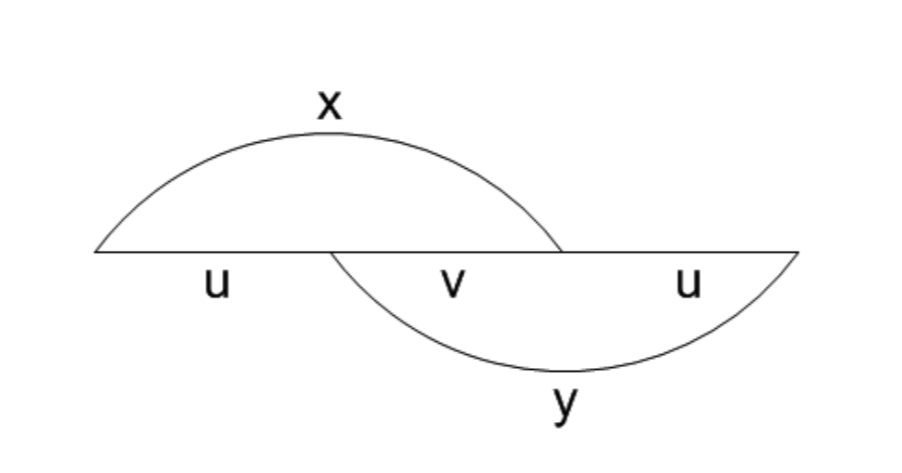
\includegraphics[scale=0.5]{1_1.png}
\caption{\textbf{Hình 1.1} \textit{Một overlap của hai từ liên hợp x và y}}
\end{figure}
\begin{flushleft}
Một tập con của $A^*$ được gọi là một \textit{ngôn ngữ} trên $A$.
Với một ngôn ngữ $X$ thuộc $A^*$, ta kí hiệp $X^*$ vị nhóm con sinh bởi $X$,
\end{flushleft}
$X^* = \{ x_1x_2...x_n | n \ge 0, x_i \in X\}$
\begin{flushleft}
Tương tự, ta kí hiệu $X^+$ nửa nhóm con sinh bởi $X$,
\end{flushleft}
$X^+ = \{ x_1x_2...x_n | n \ge 1, x_i \in X\}$
\begin{flushleft}
Ta có
\end{flushleft}
$$
\begin{cases}
    X^* - \{ \theta \} & \textit{nếu } \theta \not\in X, \\
    X^* & \textit{nếu } \theta \not\in X, \\
\end{cases}
$$
\begin{flushleft}
\hspace{10mm}Một \textit{phân tích} của một từ $\omega \in A^*$ theo các từ của $X$ cho bởi đẳng thức $\omega = x_1x_2...x_n, x_i \in X, i \ge 1$. Khi đó, ta cũng nói $\omega$ có một $X$-\textit{phân tích}. Theo định nghĩa, mỗi từ $\omega \in X^*$ có ít nhất một $X$-\textit{phân tích}. Để dễ hình dung, ta thường biểu diễn một $X$-\textit{phân tích} $\omega = x_1x_2...x_n, x_i \in X, i \ge 1$ bằng hình sau: \\
\end{flushleft}
\begin{figure}[ht]
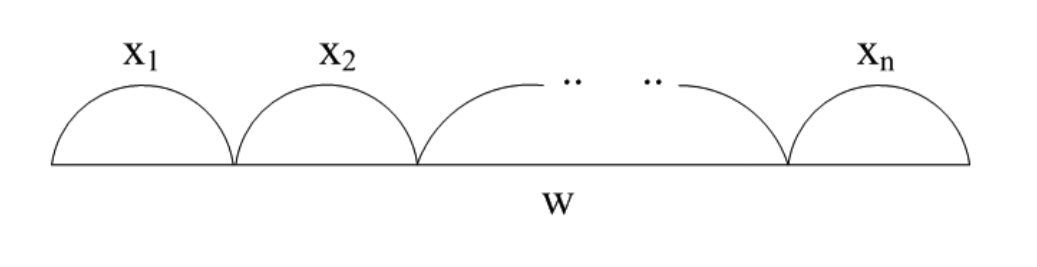
\includegraphics[scale=0.5]{1_2.png}
\caption{\textbf{Hình 1.2} \textit{Một X - phân tích từ} $\omega$}
\end{figure}
\begin{flushleft}
hspace{10mm}Cho $X, Y \subseteq A^*$ là các ngôn ngữ. \textit{Tích} của $X$ và $Y$, \textit{thương trái, thương phải} của $X$ bởi $Y$ là các ngôn ngữ được định nghĩa ở mục trước với vị nhóm $M = A^*$. với $\omega, v \in M$, ta sẽ viết $uv$ thay cho $u.v$. Khi đó:
\end{flushleft}
$XY = \{ xy|x \in X , y \in Y\}$,\\
$Y^{-1}X = \{ \omega \in A^* | y\omega \in X , y \in Y\}$,\\
$XY^{-1} = \{ \omega \in A^* | y\omega \in X , y \in Y\}$
\begin{flushleft}
Ký hiêu $u^{-1}X, Xu^{-1}$ được sử dụng khi tập $Y$ chỉ có một phần tử $Y = \{ u \}$.
\end{flushleft}
%*************************************************************************
%+ 1.3. Otomat và ngôn ngữ chính quy 
%**********************************************************
\begin{flushleft}
\section{Otomat và ngôn ngữ chính quy}
Cho A là một bảng chữ, một \textit{otomat} trên A là một bộ $\mathcal{A}$ = $(\mathcal{Q},A, \mathcal{F})$ gồm một tập hữu hạn các trạng thái Q và các tập $\mathcal{F} \subseteq Q \times A \times Q$, mỗi cung có dạng \textit{p,a,q} với \textit{p} là đỉnh đầu, $q$ là đỉnh cuối và $a$ là nhãn của cung. Ta còn biểu diễn một Otomat với \textit{tập trạng thái khởi đầu} $I \subseteq Q$ và \textit{tập trạng thái kết thúc} $T \subseteq Q$ bởi $( Q, A, \mathcal{F}, I, T )$ hoặc ngắn gọn $(Q, I, T)$ khi $A$ và $\mathcal{F}$ cố định.
\end{flushleft}
\hspace{10mm}Otomat $\mathcal{A}$ = $(Q, A, \mathcal{F})$ là \textit{hữu hạn} nếu tập trạng thái $Q$ hữu hạn.\\
\hspace{10mm}Một \textit{đường đi} trong otomat $A$ là một dãy $c$ = $(f_1, f_2, ... ,f_n)$ các cung liền nhau \\
$f_i$ = $(q_i, a_i, q_{i+1})$,  $1 \le i \le n.$
\begin{flushleft}
    \hspace{10mm}Số $n$ được gọi là \textit{độ dài} của đường đi $c$. Từ $w$ = $a_1a_2...a_n$ là \textit{nhãn} của đường đi $c$. Trạng thái $q_1$ là \textit{điểm đầu} và trạng thái $q_{n+1}$ là \textit{điểm cuối} của $c$. Để thuận tiện khi tham chiếu đến đường đi $c$, ta sử dụng ký hiệu
\end{flushleft}
$c$ : $q_1$ $\xrightarrow{w} q_{n+1}.$
\begin{flushleft}
    Quy ước, với mỗi trạng thái $q \in Q$ , có một đường đi độ dài 0, nhãn $\varepsilon$, từ $q$ đến $q$. 
\end{flushleft}
\begin{flushleft}
\hspace{10mm}Một đường đi $c : i \to t$ là \textit{đường đi thành công} nếu $i \in I$ và $t \in T$. Ngôn ngữ \textit{đoán nhận được} bởi $\mathcal{A}$ ký hiệu là $L(\mathcal{A})$, được định nghĩa là tập các nhãn của các đường đi thành công. $L(\mathcal{A})$ = $\{ w \in A^* $ | $ \exists c : i \xrightarrow{w} t, i \in I, t\in T \}$.
\end{flushleft}
\begin{flushleft}
\hspace{10mm}Một Otomat $\mathcal{A}$ = $(Q, I, T)$ là \textit{đơn định} nếu $Card(I)=1$ và nếu  
\end{flushleft}
$(p,a,q),(p,a,r) \in \mathcal{F} \Rightarrow q = r$.
\begin{flushleft}
\hspace{10mm}Vì vậy, với mỗi $P \in Q$ và $a \in A$ có nhiều nhất một trạng thái $q \in Q$ sao cho $p \xrightarrow{a} q$. Với $p \in Q$ và $a \in A$, ta định nghia 
\end{flushleft}
$p.a$ = $\begin{cases}
    q \text{  nếu  } (p,a,q ) \in \mathcal{F},\\
    \emptyset \text{  nếu  } (p,a,q) \not\in \mathcal{F}.\\ 
\end{cases}$
\begin{flushleft}
    Hàm bộ phận
\end{flushleft}
$Q \times A \to Q$
\begin{flushleft}
định nghĩa như trên được mở rộng cho từ bằng cách đặt, với mọi $q \in Q$,
\end{flushleft}
$p.\varepsilon$ = $P$,
\begin{flushleft}
và, với $w \in A^*$ và $a \in A$, 
\end{flushleft}
$p.wa$ = $(p.w).a$
\begin{flushleft}
Hàm định nghĩa như trên được gọi là \textit{hàm chuyển} của $\mathcal{A}$. Khi đó, với $I$ = $\{ i \}$ ta có
\end{flushleft}
$L(\mathcal{A})$ = $\{ w \in A^* \text{ | } i.w \in T \}$.
\begin{flushleft}
\hspace{10mm}Cho $X \subseteq A^*$ là một ngôn ngữ chính quy. Ta định nghĩa một otomat hữu hạn đặc biệt $\mathcal{A}(X)$ = $(Q, i, T)$ như sau. Các trạng thái của $\mathcal{A(X)}$ là các tập khác rỗng 
\end{flushleft}
$u^{-1}X$
\begin{flushleft}
Với $u \in A^*$. Trạng thái khởi đầu là $X$ = $\varepsilon^{-1} X$, và các trạng thái kết thúc có chứa từ rỗng. Hàm chuyển cho một trạng thái $Y$ = $u^{-1} X$ và một chữ cái $a \in A$ được cho bởi  
\end{flushleft}
$Y \xrightarrow{a} a^{-1} Y$.
\begin{flushleft}
Đây là một hàm bộ phận và ta có 
\end{flushleft}
$L(\mathcal{A(X)})$ = X.
\begin{flushleft}
\hspace{10mm}Ta biết rằng theo \hyperlink{page.78}{\textcolor{red}{5}}, otomat $\mathcal{A} (X)$ được gọi là \textit{otomat tối tiểu} của X theo nghĩa đơn định, có số trạng thái ít nhất mà đoán nhận X. 
\end{flushleft}
\begin{flushleft}
\hspace{10mm}Cho $\mathcal{A}$ = $(Q, i, T)$ là một Otomat đơn định. Ta xét tập $\mathcal{F}$ của các hàm bộ phận từ $Q$ đến Q. Các hàm này được viết về phía bên phải: nếu $q \in Q$ và $m \in \mathcal{F}$ khi đó ảnh của $q$ bởi $m$ được ký hiệu là $qm$. Hàm hợp được định nghĩa bởi 
\end{flushleft}
$q (mn) = (qm) n $
\begin{flushleft}
\hspace{10mm}Vì vậy $\mathcal{F}$ có cấu trúc vị nhóm 
\end{flushleft}
\begin{flushleft}
\hspace{10mm}Xét $\varphi$ là một ánh xạ cho tương ứng mỗi từ $w \in A^*$ một hàm bộ phận từ $Q$ đến $Q$ định nghĩa bởi 
\end{flushleft}
$q \varphi (w) $ = $q.w.$
\begin{flushleft}
    \hspace{10mm}Khi đó, ánh xạ $\varphi$ là một đồng cấu từ $A^*$ đến vị nhóm $\mathcal{F}$, và vị nhóm $\varphi (A^*) $ của $\mathcal{F}$ được gọi là \textit{vị nhóm các phép chuyển dịch} của otomat $\mathcal{A}$.\\
    \hspace{10mm}Một đồng cấu $\varphi$ từ $A^*$ đến một vị nhóm $M$ được gọi là thoả mãn ngôn ngữ $X \subseteq A^*$ nếu tồn tại $B \subseteq M$, $B$ = $\varphi(X)$ sao cho 
\end{flushleft}
$\varphi^{-1}(B)$ = $X$.
\begin{flushleft}
    \hspace{10mm}Khi đó, ta cũng nói $X$ \textit{thoả bởi} $M$ và $X$ cho bởi một bộ ba $(\varphi, M, B)$.
    \hspace{10mm}Cho $X, Y \subseteq A^*$ là các ngôn ngữ. Ta thiết lập bổ đề kỹ thuật sau đây về tính thoả được làm cơ sở xây dựng các thuật toán trên vị nhóm trong các chương trình tiếp theo.
\end{flushleft}
\begin{flushleft}
\textbf{Bổ đề 1.1} \hspace{10mm} \textit{Giả sử h:} $A^* \to M$ \textit{là một toàn cấu vị nhóm thoả X và Y và gỉa sử} $X$ = $h^{-1}(K)$, $Y$ = $h^{-1}(L)$, $h(X^+)$ = $T$ \textit{với} $K, L, T \subseteq M$. Khi đó
\end{flushleft}
$X \cup Y$ = $h^{-1}(L \cup L)$, $X \cap Y$ = $h^{-1}(K \cap L)$, $X - Y$ = $h^{-1}(K - L)$,\\
$X^{-1}Y$ = $h^{-1}(K^{-1}L)$, $XY^{-1}$ = $h^{-1}(KL^{-1})$, $(X^+)^{-1}Y$ = $h^{-1}T^{-1}L$,\\
$Y(X^+)^{-1}$ = $h^{-1}(LT^{-1})$.
\begin{flushleft}
\textit{Chứng minh}. Giả sử $X$ = $h^{-1}(K)$, $Y$ = $h^{-1}(L)$, $K, L, \subseteq P$, ta chứng mình $X \cup Y$ = $h^{-1}(K \cup L)$. \\
\hspace{10mm}Trước hết, ta chứng minh $X \cup Y \subseteq h^{-1}(K \cup L)$. Thật vậy, với mọi $w \in X \cup Y$, ta có $h(w) \in K$ hoặc $h(w) \in L$. Vậy $X \cup Y \subseteq h^{-1}(K \cup L)$. \\
\hspace{10mm}Ngược lại, ta chứng minh $h^{-1}(K \cup L) \subseteq X \cup Y$. Thật vâtj, với mọi $w \in h^{-1}(K \cup L)$, ta có $h(w) \in K \cup L$. Nghĩa là $w \in X \cup Y$. Vậy $h^{-1}(K \cup L) \subseteq X \cup Y$. \\
\hspace{10mm}Ta chứng minh tương tự cho các quan hệ $X \cap Y$ = $h^{-1}(K \cap L)$, $X - Y$ = $h^{-1}(K - L)$, $X^{-1}Y = h^{-1}(K - L)$, $X^{-1}Y$ = $h^{-1}(K^{-1}L)$ và $XY^{-1}$ = $h^{-1}(KL^{-1})$. \\
\hspace{10mm}Từ giả thiết $h(X^+)$ =$T$ và $X = h^{-1}(K)$ ta có $K^+$ = $T$. Để chứng minh $(X^+)^{-1}Y$ = $h^{-1}(T^{-1}L)$, ta chứng minh $(X^+)^{-1}Y \subseteq h^{-1}(T^{-1}L) \subseteq (X^+)^{-1}Y$.
\hspace{10mm}Trước hết, ta chứng minh $(X^+)^{-1}Y$ = $h^{-1}(T^{-1}L)$. Thật vậy, với mọi $w \in (X^+)^{-1}Y$, tồn tại $x_1, x_2, ..., x_n \in X, y \in Y$ sao cho $x_1x_2...x_nw = y$. Từ đó suy ra $h(x_1).h(x_2)...h(x_n) = h(y) \in L$. Hơn nữa, từ $h(x_i) \in K$ suy ra $h(w) \in (K^+)^{-1}L$. Vậy $w \in h^{-1}(T^{-1}L)$. \\
\end{flushleft}
Ngược lại ta chứng minh $h^{-1}(T^{-1}L) \subseteq (X^+)^{-1}$. Đặt $w \in h^{-1}(T^{-1}L)$, ta có \\
$h(w) \in T^{-1}L$ = $(K^+)^{-1}L \Leftrightarrow \exists \alpha \in K^+ : \alpha.h(w) \in L$. 
\begin{flushleft}
Từ $\alpha \in K^+$ suy ra $\alpha$ = $\alpha_1\alpha_2...\alpha_p, \alpha_i \in K, i = 1,...,o$. Từ giả thiết h là toàn cấu và $X = h^{-1}(K)$ suy ra tồn tại $x_i \in X, i = 1,...,p$ sao cho $\alpha_i$ = $h(x_i)$. Ta có $\alpha = h(x1x_2...x_p)$, khi đó $\alpha.h(w)$ = $h(x_1x_2...x_pw)$. Từ đó suy ra $x_1x_2...x_pw \in h^{-1}(L)$ = $Y$ và ta có $ư \in (X^+)^{-1}Y$. \\
\hspace{10mm}Chứng minh $Y(X^+)^{-1}$ = $h^{-1}(LT^{-1})$ tương tự.\\
Vậy chứng minh được hoàn thành.\\
\hspace{10mm}Cho $X \subseteq A^*$ là một ngôn ngữ. Với $w \in A^*$, ta định nghĩa \textit{tập ngữ cảnh}
\end{flushleft}
Context($w$) = $\{ (u,v) \in A^* \times A^* | uwv \in X \}$.
\begin{flushleft}
\hspace{10mm}\textit{Tương đẳng cú pháp} của $X$ là một quan hệ tương đương $\equiv_X$ trên $A^*$ được định nghĩa bởi 
\end{flushleft}
$w \equiv_x w' \Leftrightarrow Context(w) = Context(w')$.
\begin{flushleft}
\hspace{10mm}Tập thương của $A^*/ \equiv_x được gọi là$ \textit{Vị nhóm cú pháp} của $X$. Ta ký hiệu vị nhóm cú pháp của $X$ là $M_x$ và kí hiệu $\varphi_x$ là đồng cấu chính tắc từ $A^*$ đến $M_x$, gọi là \textit{đồng cấu cú pháp} của X.\\
\hspace{10mm}Cho $X \subseteq A^*$ là một ngôn ngữ, ta có các kết quả sau đây về tính thoả thuận theo $\varphi_x$, mối liên hệ giữa vị nhóm cú pháp của $X$ và otomat tối tiểu của $\mathcal{A}(X)$ \\
\textbf{Mệnh đề 1.1} (\hyperlink{page.80}{\textcolor{red}{5}})  Cho $X \subseteq A^*$ \textit{là một ngôn ngữ và cho} $\varphi : A^* \to M$ \textit{là một toàn cấu vị nhóm. Nếu $\varphi$ thoả mãn X thì tồn tại một đồng cấu $\psi$ từ M đến vị nhóm cú pháp $M_x$ sao cho $\varphi_x = \psi \circ \varphi$}. \\
\textbf{Mệnh đề 1.2} (\hyperlink{page.80}{\textcolor{red}{5}})  Cho $X \subseteq A^*$ \textit{là một ngôn ngữ. Vị nhóm cú pháp của X đẳng cấu với vị nhóm các phép chuyển dịch của otomat tối tiểu $\mathcal{A}(X)$}.\\
\hspace{10mm}Lớp các \textit{ngôn ngữ chính quy} trên $A^*$(trên $A^+$) được ký hiệu là $RecA^*(RecA^+)$. Ta biết rằng $RecA^*$ là lớp các ngôn ngữ sinh bởi các ngôn ngữ {$a$}, với $a$ là một chữ cái thuộc A, các phép toán Boole($\cup, \cap, - $), phép nhân và phép lặp *, và cũng là lớp các ngôn ngữ đoán nhận được bởi otomat hữu hạn, $RecA^+$ = $\{ L \in RecA^* | L \subseteq A^+ \}$. \\
Ta có\\
\textbf{Mệnh đề 1.3} (\hyperlink{page.80}{\textcolor{red}{5}})  \textit{Lớp các ngôn ngữ chính quy trên $A^*$ đóng đối với phép toán Boole: phép hợp ($\cup$), phép giao ($\cap$), phép lấy phần bù ($-$)}.\\
\hspace{10mm}Định lý sau đây đặc trưng các tính chất của otomat hữu hạn \\
\textbf{Định lý 1.1} (\hyperlink{page.80}{\textcolor{red}{5}})  Cho $X \subseteq A^*$ \textit{là một ngôn ngữ. Các mệnh đề sau đây tương đương}\\
\hspace{10mm}\textit{(i)    X là chính quy}.\\
\hspace{10mm}\textit{(ii)    X là đoán nhận bởi một otomat hữu hạn (hoặc X là đoán nhận được)}.\\
\hspace{10mm}\textit{(iii)    Otomat tối tiểu $\mathcal{A}(X)$ là hữu hạn}.\\
\hspace{10mm}\textit{(i$v$)    Họ các tập}.\\
\end{flushleft}
$u^-1X$,
\begin{flushleft}
\hspace{20mm} với $u \in A^*$, là hữu hạn.\\
\hspace{10mm}\textit{($v$)    Vị nhóm cú phép $M_x$ là hữu hạn}.\\
\hspace{10mm}\textit{($vi$)   X thoả bởi một đồng cấu từ $A^*$ đến một vị nhóm hữu hạn M}.\\
\textit{Nhận xét 1.1}   Giả sử $X \subseteq A^+ $thoả bởi một đồng cấu vị nhóm $\varphi : A^* \to M$ từ $A^*$ đến một vị nhóm hữu hạn M. Nếu X là ngôn ngữ chính quy, ta có thể chọn M là vị nhóm các phép chuyển dịch của otomat tối tiểu đoán nhận X, hoặc vị nhóm cú pháp $M_x$ hữu hạn của X. Ta gọi $m = Card(M_x)$ \textit{là chỉ số tương đẳng cú pháp} của X, hay đơn giản, \textit{m là chỉ số} của X, hoặc X có chỉ số $m$.\\
\hspace{10mm}Từ bổ đề \hyperlink{page.17}{\textcolor{blue}{1.1}} và Mệnh đề \hyperlink{page.17}{\textcolor{blue}{1.3}}, ta có \\
\textbf{Hệ quả 1.1} Cho $X, Y \subseteq A^*$ \textit{là các ngôn ngữ chính quy, P là một vị nhóm hữu hạn và $h : A^* \to P$ là một toàn cấu vị nhóm. Nếu $X$ và $Y$ cùng thoả bởi h, thì h thoả tất cả các ngôn ngữ $L \in \mathcal{A}(X, Y)$, với $\mathcal{A}(X, Y)$ là tập tất cả các ngôn ngữ sinh ra bởi X, Y nhờ thực hiện một số hữu hạn các phép toán hợp, giao, lấy phần bù, lấy thương trái và lấy thương phải.}\\
\hspace{10mm} Mệnh đề sau đây được suy từ định nghĩa cho phép ta xây dựng toàn cấu $h$ trong hệ quả trên.\\
\textbf{Mệnh đề 1.4}    \textit{Cho $X, Y \subseteq A^*$ là các ngôn ngữ chính quy $, f : A^* \to M và g : A^* \to N $ là các đồng cấu vị nhóm, f thoả X và g thoả Y. Giả sử $h : A^* \to P \subseteq M \times N$ là một toàn cấu vị nhóm cho bởi: $\forall \in A^*, h(a) = (f(a),g(a)$ và P là một vị nhóm con của $M \times N$ sinh bởi tập tất cả các phần tử $h(a), a \in A$. Khi đó h thoả đồng thời X và Y}.\\
\begin{flushleft}
\textit{Ví dụ 1.4}  Cho $\varphi : A^* \to M$ là một đồng cấu vị nhóm thoả $X, Y \subseteq A^*, A \ne \emptyset$ và cho $Y = \{ \varepsilon \}$. Ta xây dựng toàn cấu $h$ thoả cả X và Y theo một trong 2 cách sau.\\
\hspace{10mm}Cách 1. Cho $Z_2 = \{ 0,1 \}$ là vị nhóm nhân modulo 2 của các số nguyên với đơn vị 1. Rỡ tàng, $Y = \{ \varepsilon \}$ thoả bởi đồng cấu $y : A^* \to Z_2$, được định nghĩa bởi $g(\varepsilon) = 1$ và với mọi $a \in A, g(a) = 0$. Ta có thể kiểm tra X và Y = {$\varepsilon$} cùng thoả bởi toàn cấu vị nhóm\\
$h : A^* \to P \subseteq M \times Z_2$ được cho bởi $\forall a \in A, h(a)$ = $(\varphi (a) , 0), 1_p$ = $h(\varepsilon)$ = $(1_M, 1)$.\\
Đặt $\overline{K}$ = $h(A) \cup 1_P$ = $\{ (h(a), 0) | a \in A \cup 1_P \}$, tâ có $\overline{A}^*$ = $P$.
\hspace{10mm}Cách 2. Mở rộng vị nhóm $M$ thành vị nhóm $M^1$ = $M \cup \{1\}$ với $1 \not\in M$ là phần tử đơn vị mới của $M^1$ bởi điều kiện ($\textbf{1}.x = x.\textbf{1} = x, \forall x \in M^1$).
\hspace{10mm}Định nghĩa $h' : A^* \to M^1$ ta định nghĩa toàn cấu $h : A^* \to P$ = $h'(A)^* \subseteq M^1$ cho bởi $h' : h(a)$ = $h'(a), \forall a \in A, h(\varepsilon) = h'(\varepsilon) = 1$.
\section{Mã của các từ hữu hạn}
\subsection{Mã và các tính chất đại số của mã}
Trong phần này ta xem xét định nghĩa và một số tính chất quan trọng của mã. Trước hết ta nhắc lại khái niệm tích không nhập nhằng là cơ sở để xây dựng khái niệm mã.\\
\hspace{10mm}Cho A là một bảng chữ và $X, Y \subseteq A^*$ là các ngôn ngữ. Tích $XY$ là \textit{không nhập nhằng} nếu mỗi từ $w \in XY$ có duy nhất một phân tích $w = xy$ với $x \in X, y ư\in Y$.\\
\textbf{Định nghĩa 1.1}     \textit{Giả sử A là một bảng chữ hữu hạn. Tập $X \subseteq A^+ $ là mã trên A nếu với mọi $n,m \ge 1$ và với mọi $x_1x_2,...,x_n,y_1y_2,...,y_m \in X$, nếu có} 
\end{flushleft}
\end{flushleft}
$x_1x_2...x_n$ = $y_1y_2...y_m$
\begin{flushleft}
\textit{thì khi đó}
\end{flushleft}
$n = m$ và  $x_i = y_i$     với     $i = 1,...,n$.
\begin{flushleft}
Cho $X \subseteq A^*$ là một ngôn ngữ. Từ định nghĩa của mã ta suy ra các tính chất sau đây.\\
\textbf{Tính chất 1.2}      X là mã nếu mỗi từ $x \ A^*$ (t.ư $w \in X^*$) có nhiều nhất (t.ư chỉ có duy nhất) một $X$-phân tích.\\
\textbf{Tính chất 1.3}    X là mã khi và chỉ khi $X^{-1}X \cap X^*(X^*)^{-1}$ = $\{ \varepsilon \}$.
\textit{Ví dụ 1.5}  Ngôn ngữ $X = \{ ab,abb,bb \}$ trên bảng chữ $A = \{ a,b \}$ là mã. Thật vậy, giả sử X không là mã. Khi đó tồn tại một từ $w \in X^+$ có độ dài tối tiểu thừa nhập hai X-phân tích khác nhau.
\end{flushleft}
$w = x_1x_2...x_n = y_1y_2...y_m$ với $x_1 \ne y_1$
\begin{flushleft}
$(n, m \le 1, x_i, y_i \in X )$. Từ đó $x_1 \ne y_1$ suy ra $x_1$ là khúc đầu của $y_1$ hoặc ngược lại. Giả sử $x_1$ là khúc đầu của $y_1$. Với $X$ như trên, ta có $x_1 = ab$ và $y_1 = abb$. Từ đó suy ra $x_2 = bb, y_2 = bb$. Vậy $y_1 = x_1b, y_1y_2 = x_1x_2b$. Thực hiện chứng minh quy nạp theo $k \le 1,$ ta có $x_{k+1} = bb$ và $y_{k+1} = bb$. Từ đó suy ra $y_1y_2...y_{k+1}$ = $x_1x_2...x_{k+1}b$ với mọi $k \le 1$. Điều này có nghĩa là không thể có từ $w$ hữu hạn thừa nhận hai X-phân tích khác nhau, trái với giả thiết. \\
\begin{figure}[ht]
    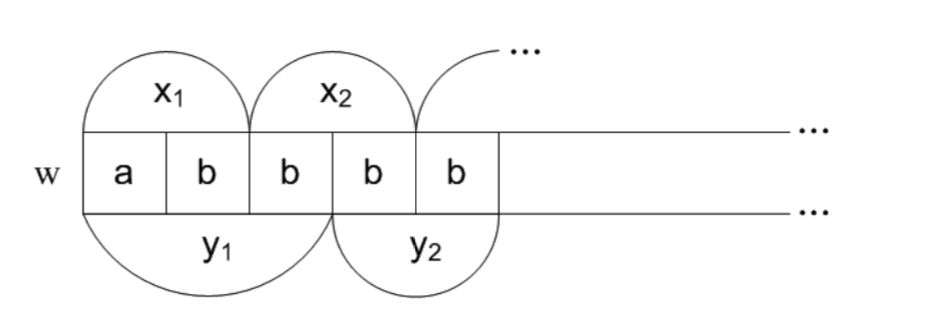
\includegraphics[scale=0.5]{1_3.png}
    \caption{ \textit{Khởi đầu một phân tích kép của từ $w$} }
\end{figure}
\textit{Ví dụ 1.6}  Cho $A = \{ a.b \}$ và $X = \{ b, abb, abbba, bbba, baabb \}$. Ngôn ngữ X không là mã vì tồn tại $w = abbbabbbaabb, w$ có hai X-phân tích khác nhau,
\end{flushleft}
$w = (abbba)(bbba(abb)$ = $(abb)(b)(abb)(baabb)$.\\
Định nghĩa mã theo cách sau đây cho phép ta diễn tả ý nghĩa của thuật ngữ \textit{mã}.
\begin{flushleft}
\textbf{Mệnh đề 1.5} (\hyperlink{page.80}{\textcolor{red}{5}})  \textit{Nếu $X \subset A^*$ là mã thì mỗi đồng cấu $\beta$ : $B^* \to A^*$ cảm sinh một song ánh từ bảng chữ B đến X là đơn cấu. Ngược lại, nếu tồn tại đơn cấu $\beta : B^* \to A^*$ sao cho X = $\beta(B)$, thì X là mã.}
\hspace{10mm}Một đơn cấu $\beta : B^* \to A^*$ với $X = \beta(B)$ được gọi là một \textit{đồng cấu mã} đối với X. Mệnh đề \hyperlink{page.20}{\textcolor{blue}{1.5}} trình bày ý nghĩa gốc củ thuật ngữ \textit{mã} vì các từ của X mã hoá các chữ cái của bảng chữ B. Thủ tục mã kết hợp một \textit{từ bản rõ} $b_1b_2...b_n (b_i \in B)$ với một \textit{từ mã} $\beta(b_1)...\beta(b_n)$ bởi sử dụng đồng cấu mã $\beta$. Sự kiện $\beta$ là đơn cấu đảm bảo từ mã được giải mã theo một cách duy nhất thành từ bản rõ ban đầu.\\
\hspace{10mm} Từ mệnh đề \hyperlink{page.20}{\textcolor{blue}{1.5}} ta có \\
\textbf{Hệ quả 1.2} (\hyperlink{page.81}{\textcolor{red}{5}})  \textit{ Giả sử $\alpha : A^* \to C^*$ là một đơn cấu. Nếu X là mã trên A, thì $\alpha(X)$ là mã trên C. Nếu Y là mã trên C, thì $\alpha^{-1}(Y)$ là mã trên A.}\\
\textbf{Hệ quả 1.3} (\hyperlink{page.81}{\textcolor{red}{5}}) \textit{Nếu $X \subset A^*$ là mã, thì khi đó $X^N$ là mã với mọi n > 0.}\\
\hspace{10mm} Ta nhắc lại rằng một vị nhóm con của $M$ của $A^*$ là \textit{tự do} khi và chỉ khi với mọi $m \in M - \{ \varepsilon \}$ co duy nhất một phân tích trong $X = (M - \{ \varepsilon \}) - (M - \{ \varepsilon \})^{2}$\hyperlink{page.81}{\textcolor{red}{18}}. Mã X cảm sinh vị nhóm con tự do $M$ của $A^*$ được gọi là cơ sở của $M$. Mối liên hệ giữa mã và vị nhóm con sinh bởi mã được thiết lập qua các tính chất sau đây.
\textbf{Mệnh đề 1.6} (\hyperlink{page.80}{\textcolor{red}{5}}) \textit{Giả sử A là một bảng chữ. Khi đó, mỗi vị nhóm con M của $A^*$ có một tập sinh cực tiểu duy nhất X = (M - $\{ \varepsilon \}$) - (M - $\{ \varepsilon \}^{2}$)}.\\
\textit{Ví dụ 1.7}  Tập M = $\{ a^i, i \in \mathbb{N}, i \not\in 1 \}$ là một vị nhóm con của $A^*$ với $A = \{ a,b \}$. Cơ sở của $M$ là $X = \{ a^2, a^3 \}$. Tuy nhiên, $M$ không phải là một vị nhóm con tự do vì $a^6 \in M$ có hai phân tích khác nhau trong $X, a^6 = a^2.a^2.a^2 = a^3.a^3.$ \\
\textbf{Mệnh đề 1.7} (\hyperlink{page.81}{\textcolor{red}{5}}) \textit{Nếu M là một vị nhóm con tự do của $A^*$, thì khi đó tập sinh cực tiểu của M là mã. Ngược lại nếu $X \subset A^*$ là mã, thì vị nhóm con của $X^*$ của $A^*$ là tự do có tập sinh cực tiểu $X$}.\\
\textbf{Mệnh đề 1.7} (\hyperlink{page.81}{\textcolor{red}{5}})  \textit{Giả sử X và Y là các mã trên A. Nếu $X^* = Y^*$, thì khi đó X = Y.} \\
\subsection{Độ trễ của giả mã}
Khái niệm độ trễ của giả mã được giới thiệu nhằm mở rộng các khái niệm của mã \textit{prefix} cho trường hợp mã thông thường. Ta biết rằng lớp mã prefix có độ trễ 0, do đó mã có độ trễ giải mã giới nội là trường hợp tổng quát của mã prefix. Ta nhắc lại ngôn ngữ $X \subset A^*$ là mã prefix khi và chỉ khi $X$ là mã và $X$ là tập prefix. khái niệm độ trễ của giải mã đươc định nghĩa như sau: \\
\textbf{Định nghĩa 1.2}\text{   } \textit{Giả sử X là một tập con của $A^+$. Khi đó $X$ được gọi là có độ trễ giải mã hữu hạn nếu có một số nguyên $d \ge 0$ sao cho }  
\end{flushleft}
$\forall x, x' \in X , \forall y \in X^d , \forall u \in A^* , xyu \in x'X^* \rightarrow x = x'$. (1.1)
\begin{flushleft}
\hspace{10mm}Dễ thấy rằng nếu hệ thức (\hyperlink{page.21}{\textcolor{blue}{1.1}}) thoả mãn với $d$ nào đó thì nó cũng đúng với mọi $d' \ge d$. Nếu $X$ có độ trễ giải mã hữu hạn thì số nguyên nhỏ nhất thoả hệ thức (\hyperlink{page.21}{\textcolor{blue}{1.1}}) được gọi là \textit{độ trễ giải mã yếu} của X. 
\textit{Ví dụ 1.8}  Cho $A = \{ a,b \}$. Khi đó tập $X = \{ ab, abb, baab \}$ có độ trễ giải mã $d = 1$. và tập $Y = \{ a, ab, b^2 \}$ có độ trễ giải mã vô hạn.\\
\hspace{10mm}Ta có mệnh đề sau đây về mối quan hệ giữa mã và độ trễ giải mã. \\
\textbf{Mệnh đề 1.8} (\hyperlink{page.81}{\textcolor{red}{5}}) \textit{Cho $X \subset A^*$}. Nếu X có độ trễ giải mã hữu hạn thì X là mã.\\
\textit{Ví dụ 1.9.} Cho tập $X$ như ví dụ \hyperlink{page.21}{\textcolor{blue}{1.8}}. Bằng định nghĩa, ta có thể kiểm tra tập X là mã. \\
\subsection{Tiêu chuẩn kiểm định mã}
Thuật toán kiểm định mã là một thuật toán cốt lõi và kinh điển trong lý thuyết mã. Cần thiết cho các nghiên cứu về mã truyền thống và các hình thức mã mới. Trong phần này, ta nhắc lại thuật toán kinh điển Sardinas-Patterson.\\
\hspace{10mm}Cho một ngôn ngữ $X \subseteq A^+$, ta xem xét các tập phần dư $U_i$ kết hợp với $X$ được định nghĩa đệ quy như sau:
\end{flushleft} 
$
    U_1 = X^{-1}X = \{ \varepsilon \}
$ \\
\begin{flushright}
    (1.2)
\end{flushright}
$
    U_{i+1} = (U_i)^{-1}X \cup X^{-1}U_i, i \ge 1. 
$
\begin{flushleft}
\hspace{10mm}Định lý cơ bản sau đây của Sardinas-Patterson cung cấp một tiêu chuẩn kiểm định mã.
\textbf{Định lý 1.2} (\hyperlink{page.81}{\textcolor{red}{5}}) \textit{Tập $X \subseteq A^+$ là mã khi và chỉ khi các tập $U_i$ được định nghĩa theo công thức (\hyperlink{page.21}{\textcolor{blue}{1.2}}) không chứa từ rỗng.}
\textit{Nhận xét 1.2}   Như một hệ quả của mệnh đề \hyperlink{page.18}{\textcolor{blue}{1.4}} Mục (\hyperlink{page.13}{\textcolor{blue}{1.3}}), trong trường hợp $X$ là ngôn ngữ chính quy, lấy $M$ là $M_x$ - vị nhóm cú pháp hữu hạn của $X$, ta suy nghĩa ra rằng tất cả các tập $U_i$ thuộc vào tập hữu hạn $\mathcal{A}(X,Y)$ sinh ra bởi $X,Y$ và đóng đối với các phép toán hợp, giao, lấy phần bù, lấy thương trái và lấy thương phải. $Card(\mathcal{A}(X,Y)) \le 2^{2.m}$, với $m$ là chỉ số của $X$.
\textit{Nhận xét 1.3}   Cho một ngôn ngữ chính quy $X \subseteq A^*$ có chỉ số m, đặt $Y = \{ \varepsilon \}$. Từ đó vị nhóm P được xác định như Ví dụ \hyperlink{page.18}{\textcolor{blue}{1.4}} (Cách 1), cỡ của $P$ là $2.m$, khi đó cỡ của $\mathcal{A}(X,Y)$ là $2^{2.m}$ và từ tính chất $U_i \subseteq \mathcal{A}(X,Y), \forall i \ge 1$, ta suy ra rằng số bước tính toán trong tiêu chuẩn Sardinas-Patterson chính là số các tập $U_i$ khác nhau, tối đa là $2^{2.m}$.
\hspace{10mm}Nhận xét \hyperlink{page.13}{\textcolor{blue}{1.3}} khẳng định Định lý \hyperlink{page.21}{\textcolor{blue}{1.2}} cung cấp cho ta một thuật toán kiểm định một ngôn ngữ chính quy cho trước có là mã không.
\textit{Ví dụ 1.10}     Cho $A = \{ a,b \}$ và $X = \{ b, abb, abbba, bbba, baabb \}$. Tập X không là mã vì tồn tại từ $w = abbbabbbaabb, w$ có hai phân tích khác nhau trong X,    
\end{flushleft}
$w = (abbba)(bbba)(abb) = (abb)(b)(abb)(baabb)$.
\begin{flushleft}
\hspace{10mm}Sử dụng thuật toán kiểm tra mã, ta có 
\end{flushleft}
\hspace{10mm}$U_1 = \{ ba, aabb, ba \},$     $U_2 = \{ a, ba, abb \}$,   $U_3 \{ \varepsilon, a, ba, bb, bbba, abb \}$.
\begin{flushleft}
\hspace{10mm}Vì $\varepsilon \in U_3$, suy ra X không là mã.
\textit{Nhận xét 1.4}   Giả sử $V_i$ ($i \ge 1$), $V_1 \subseteq V_2 \subseteq ... \subseteq A^*$ là một dãy tăng bất kỳ sao cho mọi tập $V_i$ cùng thoả bởi một toàn cấu vị nhóm $h : A^* \to P$, với $P$ là một vị nhóm hữu hạn. Khi đó tồn tại một dãy tăng $K_1 \subseteq K_2 \subseteq ... \subseteq P$ sao cho $V_i = h^{-1}(K_i)$ với $i = 1,2....$ Dãy tăng này là hữu hạn và tổng số phần tử của nó không vượt quá $Card(P)$. Nhận xét này cung cấp một kỹ thuật để ta xây dựng các tiêu chuẩn kiểm định mã mới.
\end{flushleft}
\begin{flushleft}
\section{Mã luân phiên và mã của các từ định biên}
\subsection{Mã luân phiên}
Mã luân phiên có thể được xem là một sự mở rộng của biểu diễn mã, nó được định nghĩa trên một cặp ngôn ngữ thay vì một ngôn ngữ như mã truyền thống (xem [\hyperlink{page.81}{\textcolor{red}{14}}; \hyperlink{page.81}{\textcolor{red}{15}}; \hyperlink{page.81}{\textcolor{red}{23}}; \hyperlink{page.81}{\textcolor{red}{32}}; \hyperlink{page.81}{\textcolor{red}{35}}]). Từ một cặp ngôn ngữ $X, Y$ cho trước, khái niệm \textit{phân tích luân phiên mã luân phiên} theo X,Y được định nghĩa như sau: \\
\textbf{Định nghĩa 1.3} (\hyperlink{page.81}{\textcolor{red}{32}}) \textit{Giả sử A là một bảng chữ, $X, Y \subseteq A^+ , w \in A^+$. Khi đó, \\
\hspace{10mm}(i) từ $w$ có một phân tích luân phiên theo ($X, Y$) nếu $w = u_1u_2...u_n (n \ge 2)$, trong đó $ư_1 \in X$, nếu $u+i \in X$ thì $u_{i+1} \in Y$ và nếu $u_i \in Y thì u_{i+1} \in X $ với $ i = 1,....,n-1$.
\hspace{10mm}(ii) từ $w$ có một phân tích luân phiên theo $\{ X, Y \}$ nếu $w$ có một phân tích luân phiên theo $(X, Y)$ hoặc $(Y, X)$.
\hspace{10mm}(iii)hai phân tích luân phiên theo $\{ X, Y \}$ được gọi là cùng kiểu trái (t.ư. cùng kiểu phải) nếu chúng cùng bắt đầu (t.ư. kết thúc) với các từ trong $X$ hoặc trong $Y$.
\hspace{10mm}(iv)  hai phân tích luân phiên theo $\{ X, Y \}$ được gọi là cùng kiểu nếu chúng là cùng kiểu trái và cùng kiểu phải.
}


\end{flushleft}
%*************************************************************************
%+ 1.3. Bai toan quy hoach tuyen tinh va bai toan doi ngau.

%**********************************************************
\section{Bài toán quy hoạch tuyến tính gốc và đối ngẫu}
%+ -------------------------------------------------------------------------------------------
%+ 1.2.1. Bai toan quy hoach tuyen tinh va bai toan doi ngau.
\subsection{Bài toán quy hoạch tuyến tính gốc và đối ngẫu.}
Bài toán quy hoạch tuyến tính (QHTT) tổng quát có thể được phát biểu dưới dạng:
\begin{align}\label{eq.1.2.1}
&\min (\max) \set{ f(x):=\sum_{j=1}^n c_jx_j } \\
&\text{thỏa mãn: } D:= \begin{cases}
\sum_{j=1}^na_{ij}x_j = b_i,\quad i=1\dots, m_1,\\
\sum_{j=1}^na_{ij}x_j \leq b_i,\quad i=m_1+1\dots, m_2,\\
\sum_{j=1}^na_{ij}x_j \geq b_i,\quad i=m_2+1\dots, m,\\
l_j\leq x_j\leq u_j,\quad j=1,\dots, n.
\end{cases}\notag
\end{align}
trong đó $x_j$ gọi là các biến, $c_j$ gọi là thành phần của véc tơ hệ số hàm mục tiêu (hàm giá), $a_{ij}$ gọi là hệ số ràng buộc, $b_i$ gọi là hệ số vế phải, $l_j < u_j$ làn lượt gọi là các cận dưới và cận trên (giới hạn dưới và trên) của biến $x_j$ ($i=1,\dots, m, j=1,\dots, n$).

Để nghiên cứu tính chất và các phương pháp giải bài toán quy hoạch tuyến tính \eqref{eq.1.2.1} người ta thường chuyển bài toán này về một trong hai dạng chính tắc và chuẩn tắc. Trong khóa luận này chỉ để cập đến bài toán quy hoạch tuyến tính dạng chính tắc như sau:
\begin{align}\label{eq.1.2.2}
&\min \set{ f(x):= c^Tx} \notag\\
&\text{thỏa mãn: } D_p := \begin{cases}
Ax=b\\
x\geq 0.
\end{cases}
\end{align}

trong đó $x=(x_1,\dots, x_n)^T$ gọi là các biến cần tối ưu, $c=(c_1,\dots, c_n)^T$ là véc tơ hàm mục tiêu, ma trận $A=(a_{ij})_{m\times n}$ là ma trận hệ số ràng buộc và $b=(b_1,\dots, b_m)^T$ gọi là véc tơ vế phải. Như thông thường, hàm $f$ gọi là hàm mục tiêu, tập $D_p$ gọi là tập ràng buộc. Ma trận $A$ được giả thiết là có hạng đủ, $\text{rank}A = m\leq n$ và bài toán \eqref{eq.1.2.2} gọi là bài toán QHTT gốc, ký hiệu là (P).

Một điểm $x\in D_p$ gọi là một điểm (hay phương án) chấp nhận được. Điểm $x^{*}\in D_p$ gọi là nghiệm (hay phương án tối ưu) của bài toán \eqref{eq.1.2.2} nếu $f(x^{*})\leq f(x)$ với mọi $x\in D_p$. Vì $D_p$ là tập lồi đa diện, nên $x\in D_p$ là đỉnh của $D_p$ thì $x$ gọi là phương án cực biên (phương án cơ sở). Nếu $x^{*}$ là điểm cực biên (đỉnh) của $D_p$ và tối ưu thì $x^{*}$ gọi là phương án cực biên tối ưu.

Cho một phương án cơ sở (hay một đỉnh) $x$, ký hiệu $J_{+}(x) := \set{j\in\set{1,\dots, n}: x_j > 0}$ gọi là tập chỉ số cơ sở của $x$. Nếu $|J_+(x)|=m$ thì $x$ gọi là phương án không suy biến, còn nếu $|J_+(x)| < m$ thì $x$ gọi là phương án suy biến. Theo định lý \ref{th.1.1.2} thì tập hợp các véc tơ
\begin{align}\label{eq.1.2.2a}
B_+(x) := \set{A_j,\;|; j\in J_+(x)}
\end{align}
gồm các véc tơ cột của $A$ sẽ là một hệ độc lập tuyến tính. Nếu $r:=|J_+(x)| < m$ thì ta bổ sung thêm $m-r$ véc tơ còn lại của $A$ vào $B_+(x)$ sao cho ta thu được hệ gồm $m$ véc tơ cột của $A$ độc lập tuyến tính, ký hiệu là $B(x)$. Hệ véc tơ $B(x)$ gọi là hệ véc tơ cơ sở (hay gọi tắt là cơ sở) của phương án cực biên $x$. Thông thường để ngắn gọi, người ta thường gọi $J(x)$ là tập chỉ số cơ sở thay cho gọi cơ sở $B(x)$.

Lập hàm Lagrange cho bài toán QHTT gốc (P) như sau: 
\begin{align}\label{eq.1.2.3}
L(x, y, s) := c^Tx + y^T(b-Ax) + s^Tx
\end{align}
trong đó $y$ và $s\geq 0$ là các nhân tử Lagrange. Khi đó bài toán đối ngẫu (dạng Lagrange) của bài toán gốc (P) sẽ có dạng (sẽ ký hiệu là (D)):
\begin{align}\label{eq.1.2.4}
&\max\set{g(y,s) := b^Ty } \notag\\
&\text{thỏa mãn: }D_d:=\begin{cases}
A^Ty + s = c\\
s\geq 0.
\end{cases}
\end{align}
Biến $s$ gọi là biến bù, $g$ gọi là hàm mục tiêu đối ngẫu và $D_d$ gọi là miền ràng buộc đối ngẫu. Hiển nhiên $D_d$ cũng là tập lồi đa diện và bài toán \eqref{eq.1.2.4} cũng là bài toán QHTT.

Với mọi bộ ba $(x, y, s)$ sao cho $x\in D_p$ và $(y, s)\in D_d$ ta đặt
\begin{align}\label{eq.1.2.3}
\tau(x,y, s) := f(x) - g(y, s) = s^Tx,
\end{align}
gọi là khoảng trống đối ngẫu. Theo định lý đối ngẫu yếu thì $\tau(x,y,s)\geq 0$, và nếu $\tau(x,y,s)=0$ thì $(x,y,s)$ sẽ là nghiệm của cặp bài toán gốc đối ngẫu (P)-(D). 
Còn theo định lý đối ngẫu mạnh thì nếu $x^{*}$ là nghiệm tối ưu của bài toán gốc (P) thì sẽ tồn tại nghiệm tối ưu $(y^{*},s^{*})$ của bài toán đối ngẫu (D) sao cho $\tau^{*}=\tau(x^{*}, y^{*}, s^{*}) = 0$ và ngược lại.

%+ -------------------------------------------------------------------------------------------
%+ 1.2.2. Phuong phap don hinh giai bai toan quy hoach tuyen tinh.
\subsection{Phương pháp đơn hình giải bài toán QHTT.}
Một trong những phương pháp nổi tiếng và hiệu quả là phương pháp đơn hình, được G. B. Dantzig phát minh ra năm 1947. Phần này sẽ trình bày tóm tắt lại tư tưởng cơ bản và nội dung của phương pháp đơn hình mà sẽ sử dụng chính trong khóa luận.

Trước hết ta chỉ ra một tính chất quan trọng của bài toán quy hoạch tuyến tính là nghiệm sẽ nằm ở điểm cực biên.
%+ Bo de 1.2.1.
\begin{lemma}\label{le.1.2.1}
Giả sử bài toán QHTT gốc \eqref{eq.1.2.2} có nghiệm tối ưu thì nó sẽ có nghiệm tối ưu $x^{*}$ nằm ở đỉnh.
\end{lemma}

Do tính chất đặc biệt của bài toán QHTT nên thuật toán đơn hình đã tận dụng rất hiệu quả các tính chất này để tạo ra một thuật toán rất hiệu quả. 
Đặc biệt là các tính chất:
\begin{itemize}
\item Miền ràng buộc của bài toán QHTT là một tập lồi đa diện với số điểm cực biên là hữu hạn.
\item Nếu bài toán QHTT có nghiệm tối ưu thì sẽ có nghiệm tối ưu nằm ở đỉnh.
\end{itemize}
Ý tưởng của thuật toán đơn hình mô tả như sau:
\begin{itemize}
\item[]{\it Bước 1: } Xuất phát từ một đỉnh $x^0$ của miền ràng buộc.
\item[]{\it Bước 2: } Nếu $x^0$ là nghiệm tối ưu, dừng thuật toán. Nếu không chuyển sang Bước 3.
\item[]{\it Bước 3: } Từ $x^0$ tìm cách di chuyển đến đỉnh kề tiếp theo của miền ràng buộc tốt hơn đỉnh $x^0$ (theo nghĩa giá trị hàm mục tiêu nhỏ hơn).
\item[]{\it Bước 4: } Lặp lại Bước 2, 3 với $x^0$ thay bằng $x^1$.
\end{itemize}
Do số đỉnh của miền ràng buộc là hữu hạn, nên nếu bài toán có nghiệm, sau hữu hạn bước ta sẽ tìm được đỉnh tối ưu.
Có nhiều vấn đề cần giải quyết trong phương pháp đơn hình, bao gồm:
\begin{itemize}
\item Tìm đỉnh xuất phát, vấn đề này thường được giải quyết dựa vào phương pháp hai pha hoặc đánh thuế (hai phương pháp này cũng cho biết miền ràng buộc có rỗng hay không).
\item Kiểm tra bài toán có nghiệm hay vô nghiệm (có bị chặn dưới hay không).
\item Kiểm tra đỉnh $x^0$ có là tối ưu hay không?
\item Từ đỉnh $x^0$ làm thế nào di chuyển đến đỉnh $x^1$ tốt hơn $x^0$?
\end{itemize}

Với ý tưởng như trên, thuật toán đơn hình được mô tả như sau:

\noindent{\bf Thuật toán đơn hình.}
\begin{itemize}
\item {\bf Đầu vào: } Ma trận $A=(a_{ij})_{m\times n}$, véc tơ $b$, véc tơ $c$. Phương án cơ sở $x^0$ và cơ sở tương ứng $J(x^0)$. 
\item {\bf Đầu ra: } Phương án cơ sở tối ưu $x^{*}$ và giá trị mục tiêu tối ưu $f(x^{*})$ hoặc chỉ ra bài toán không có nghiệm tối ưu (tức là hàm mục tiêu không bị chặn dưới).
\item {\bf Thuật toán:}
\begin{itemize}
\item[]{\bf Bước khởi tạo:} 
\begin{enumerate}
\item Tìm một phương án cơ sở xuất phát $x^0$ ứng với cơ sở xuất phát $J_0:=B(x^0)$.
\item Tính các hệ số khai triển $Z=(z_{jk})$ và các ước lượng $\Delta_k$ theo các công thức tương ứng sau
$$
\begin{cases}
A_k = \sum_{j\in J_0}z_{jk}A_j\quad \forall j=\overline{1, n}\\
\Delta_k = \sum_{j\in J_0}z_{jk}c_j - c_k\quad \forall k\notin J_0\\
\Delta_k = 0\quad \forall k\in J_0
\end{cases}
$$
\end{enumerate}

\item[]{\bf Bước 1: } {\it Kiểm tra tiêu chuẩn tối ưu.}
\begin{enumerate}
\item Nếu $\Delta_k\leq 0$ với mọi $k\notin J_0$ thì $x^0$ là phương án tối ưu. Kết thúc thuật toán.
\item Nếu $\exists\Delta_k > 0$, chuyển sang bước 2.
\end{enumerate}

\item[]{\bf Bước 2: }{\it Kiểm tra tính bị chặn của hàm mục tiêu}.\\
Với mỗi $k\notin J_0$ mà $\Delta_k > 0$  ta kiểm tra các hệ số khai triển $Z_k = (z_{jk})$.\\
\begin{enumerate}
\item Nếu có một $\Delta_k>0$ mà tất cả các hệ số khai triển $z_{jk}\leq 0,\;(\forall j\in J_0)$ thì kết luận hàm mục tiêu không bị chặn dưới. Bài toán không có phương án hữu hạn. Kết thúc thuật toán.\\
\item Nếu với mọi $k\notin J_0$ mà tồn tại ít nhất một hệ số $z_{jk}>0$ thì tiến hành tìm phương án mới $x^1$ tốt hơn $x^0$ bằng cách chuyển sang bước 3.
\end{enumerate}
\item[]{\bf Bước 3: }{\it Tìm phương án mới}
\begin{enumerate}
\item Chọn véc tơ $A_s$ đưa vào cơ sở: Có thể bất kỳ $s\notin J^)$ sao cho $\Delta_s>0$. Thông thường chọn $s$ sao cho $\Delta_s$ lớn nhất
$$
\Delta_s = \max\set{\Delta_k > 0\;|\; k\notin J_0}
$$
\item Chọn véc tơ $A_r$ đưa ra khỏi cơ sở theo quy tắc:
$$
\theta := \dfrac{x^0_{r}}{z_{rs}} = \min\set{\dfrac{x^0_j}{z_{js}}\;|\; z_{js} > 0}
$$
\item Tính phương án mới $x^1$ và giá trị hàm mục tiêu mới theo công thức:
\begin{align*}
&x^1=\begin{cases}
0\quad\text{với}\quad k\notin J_0, k\neq s\\
\frac{x^0_r}{z_{rs}}\quad\text{với}\quad k = s\\
x^0_j - \frac{x^0_r}{z_{rs}}z_{js} \quad\text{với}\quad j\in J_0
\end{cases}\\
&f(x^1) = f(x^0) - \frac{x^0_r}{z_{rs}}\Delta_s
\end{align*}
\end{enumerate}
\item[]{\bf Bước 4:} Tính các hệ số khai triển và ước lượng mới theo công thức
\begin{align*}
&z_{jk}^1 = \begin{cases}
\frac{z_{rk}}{z_{rs}}\quad \text{nếu}\quad j=s\\
z_{jk} - \frac{z_{rk}}{z_{rs}}z_{js}\quad \text{nếu}\quad j\in J_0, j=r\\
\end{cases}\\
&\Delta^1_k = \Delta_k - \frac{z_{rk}}{z_rs}\Delta_s
\end{align*}
\item[]{\bf Bước 5:} Quay về bước 1 với phương án cơ sở mới $x^1$ và cơ sở mới $J_1:=J(x^1)$.
\end{itemize}
\end{itemize}
Để thuật tiện cho việc "thực hành" thuật toán đơn hình giải bài toán QHTT dạng chuẩn tắc. Ta sử dụng một bảng gọi là {\bf Bảng đơn hình} gồm $n+3$ cột và $m+3$ hàng như sau:
\begin{center}
\begin{tabular}{|c|c|c|c|c|c|c|c|c|}
 \hline
Cơ sở&$c_J$&Phương án&$1$&$2$&$\cdots$&$k$ & $\cdots$ & $n$ \\ 
$J$&& $x_J$&  $c_1$& $c_2$& $\cdots$& $c_k$& $\cdots$ & $c_n$ \\ \hline
$J_1$     & $c_{j_1}$  & $x_{j_1}$   &  $z_{j_11}$  & $z_{j_12}$  & $\cdots$    & $z_{j_13}$  & $\cdots$ & $z_{j_1n}$\\
$J_2$     & $c_{j_2}$  & $x_{j_2}$   &  $z_{j_21}$  & $z_{j_22}$  & $\cdots$    & $z_{j_23}$  & $\cdots$ & $z_{j_2n}$\\
$\vdots$ & $\vdots$   & $\vdots$   &$\vdots$       & $\vdots$     &$\vdots$    &$\vdots$      & $\vdots$ & $\vdots$\\
$J_m$    & $c_{j_m}$ & $x_{j_m}$ &$z_{j_m1}$   & $z_{j_m2}$  & $\cdots$   & $z_{j_m3}$ & $\cdots$ & $z_{j_mn}$\\ \hline
              &                & $f(x)$       & $\Delta_1$   & $\Delta_2$  & $\cdots$   & $\Delta_k$  & $\cdots$ & $\Delta_n$ \\ \hline
\end{tabular}
\end{center}
Lưu ý phần bảng dành cho các hệ số khai triển $z_{jk}$:
\begin{itemize}
\item Các cột ứng với các $j\in J_0$ sẽ là các véc tơ đơn vị với hệ số $1$ nằm trên dòng với chỉ số $j$.
\item Với $k\notin J_0$ thì cột $k$ của bàng đơn hình là hệ số khai triển của $A_k$ của ma trận $A$ theo cơ sở $J_0$. Ta ký hiệu cột này là $Z_k$ nghĩa là $A_k = B_{J_0}Z_k$ hay $Z_k =(B_{J_0})^{-1}A_k$, ở đây $B_{J_0}$ là ma trận cơ sở ($B_{J_0}=\set{A_j\;|\;j\in J_0}$. 

Đặc biệt khi ta chọn được một ma trận $B_{J_0}$ có dạng ma trận đơn vị thì hệ số khai triển trên các cột $j$ với $j\in J_0$ sẽ chính là cột véc tơ đơn vị $z^{jk} = e_j$, còn các hệ số khai triển trên các cột $k\notin J_0$ chính là $z_{jk} = A_k$.
\item Dòng ước lượng là dòng cuối cùng của bảng và được tính bởi$\Delta_k = c^T_{J_0}Z_k -c_k$ và $\Delta_j=0, (\forall j\in J_0)$.
\item Giá trị hàm mục tiêu chính là $f(x) = c^T_{J_0}x_{J^)}$.
\end{itemize}

Thuật toán nêu trên gọi là thuật toán đơn hình gốc, ngoài ra người ta còn xây dựng các thuật toán đơn hình khác như: thuật toán đơn hình đối ngẫu, thuật toán đơn hình gốc đối ngẫu. Một số phiên bản khác của thuật toán đơn hình cũng được đề cập trong các tài liệu về QHTT.

Một trong những chi tiết quan trọng trong phương pháp đơn hình là: {\it Từ nghiệm $x^{*}$ của bài toán gốc (P), ta có xây dựng lại được nghiệm đối ngẫu hay không?}. Phương pháp đơn hình gốc - đối ngẫu sẽ cho phép thu được bộ ba nghiệm $(x^{*}, y^{*}, s^{*})$ cho cặp bài toán gốc, đối ngẫu. Trên thực tế, ta có thể xuất phát từ nghiệm của bài toán gốc (P) là $x^{*}$ với cơ sở $A_{J^{*}}$, ta có thể thu được nghiệm của bài toán đối ngẫu (D) như sau:
\begin{itemize}
\item Giả sử $x^{*}$ là nghiệm của bài toán gốc (P) ứng với cơ sở tối ưu $A_{J^{*}}$. Khi đó ta có:
$$
x_{J^{*}}^{*} = A_{J^{*}}^{-1}b,
$$
với $x_{J^{*}}^{*} = (x^{*}_j)_{j\in J^{*}}$ và $(x^{*}_j)_{j\in J^{*}} = (0)$.
\item Khi đó $A_{J^{*}}$ cũng sẽ là cơ sở đối ngẫu của bài toán đối ngẫu (D) và nghiệm đối ngẫu $(y^{*}, s^{*})$ được tính theo công thức:
$$
y^{*} = (A_{J^{*}}^{-1})^Tc_{J^{*}}, \quad s^{*} = c - A^Ty^{*},
$$
trong đó $c_{J^{*}} = (c_j)_{j\in J^{*}}$.
\item Khi đó khoảng trống đối ngẫu sẽ là: $\tau^{*} = (x^{*})^Ts^{*} = 0$. Theo định lý về độ lệch bù thì nếu $x^{*}_j>0$ thì $s^{*}_j=0$, do đó dễ thấy $s^{*}_{J^{*}} = 0$.
\end{itemize}

Trong thực tế, bài toán QHTT thường không phải là bài toán dạng chuẩn tắc với véc tơ vế phải $b$ không âm, nên ta không thể có ngay được phương án xuất phát $x^0$ để thực hiện phương pháp đơn hình. Do vậy người ta thường sử dụng một trong hai phương pháp: Phương pháp đơn hình hai pha và phương pháp đánh thuế. Trong khóa luận này sẽ sử dụng phương pháp đơn hình hai pha với nội dung được tóm tắt như sau:

Trước hết, đối với bài toán gốc (P), không mất tính tổng quát ta có thể xem các $b_i\geq 0$ với mọi $i=\overline{1,m}$ . Nếu trái lại ta nhân hai vế của ràng buộc thứ $i$ với $-1$. Ta lập bài toán phụ sau
\begin{align}\label{eq.1.2.5}
&\min\set{f_a(u) := \sum_{j=1}^mu_{n+j}}\\
&\text{thoả mãn}\; D_a := \begin{cases}
\sum_{j=1}^na_{ij}x_j + u_{n+i} = b_i,\quad (i=\overline{1,m})\\
x_j\geq 0,\quad (j=\overline{1,n})\\
u_{n+i}\geq 0,\quad (i=\overline{1,m})
\end{cases}\notag
\end{align}
Các biến $u_{n+i}$ với $(i=\overline{1,m})$ gọi là các biến giả. 

Nếu ta ký hiệu $e = (1,1,\dots,1)^T$ là véc tơ gồm $m$ thành phần là $1$, $u=(u_{n+1},u_{n+2},\dots, u_{n+m})^T$ và $E$ là ma trận đơn vị cấp $m$ thì ta có thể viết bài toán trên dưới dạng
\begin{align}\label{eq.1.2.6}
&\min\set{f_a(u) := e^Tu}\\
&\text{thoả mãn}\; D_a := \begin{cases}
Ax + Eu = b\\
x\geq 0, u\geq 0
\end{cases}\notag
\end{align}
Khi đó, quan hệ giữa hai bài toán \eqref{eq.1.2.5} và \eqref{eq.1.2.6} được chỉ ra như sau:
\begin{itemize}
\item Bài toán \eqref{eq.1.2.6} có một phương án cơ sở xuất phát là $(x,u)^T:=(0, b)^T$.
\item Bài toán \eqref{eq.1.2.2} có phương án chấp nhận được khi và chỉ khi bài toán phụ \eqref{eq.1.2.6} có phương án tối ưu $(\overline{x},\overline{u})^T$ với tất cả các biến giả $\overline{u}_{n+i}=0,\; (i=\overline{1,m}$.
\end{itemize}
Do đó phương pháp đơn hình hai pha được thực hiện như sau:
\begin{itemize}
\item[]{\it Pha 1: } Lập bài toán phụ cho bài toán (P), giải bài toán phụ bằng phương pháp đơn hình. Nếu bài toán phụ vô nghiệm hoặc có nghiệm không là nghiệm chấp nhận của bài toán (P), dừng thuật toán. Ngược lại, chuyển sang pha 2.
\item[]{\it Pha 2: } Sử dụng thuật toán đơn hình giải bài toán (P) với phương án xuất phát thu được từ pha 1.
\end{itemize}

%*******************************************************************
%+ 1.3. Luu tru va xu ly ma tran kich thuoc lon.
%******************************************************************
\section{Bài toán QHTT kích thước lớn}
%+ -------------------------------------------------------------------------------------------
%+ 1.2.1. Ma tran thua va van de luu tru.
\subsection{Ma trận thưa và vấn đề lưu trữ ma trận thưa kích thước lớn}.
Các bài toán QHTT trong thực tế ứng dụng thường có kích thước lớn. Bài toán QHTT có thể xuất hiện từ các lĩnh vực ứng dụng trực tiếp như: giao thông vận tải, xây dựng kế hoạch sản xuất, chế biến, quản lý nhân lực... Ngoài ra bài toán QHTT có thể xuất hiện trong các phương pháp toán học và tin học như một bài toán phụ, chẳng hạn xuất hiện trong các phương pháp tuyến tính hóa của quy hoạch phi tuyến, trong các phương pháp nhánh và cận... Các bài toán xuất hiện như thế thường có kích thước lớn, thậm chí là rất lớn. Tuy nhiên có một thuận lợi ở đây là ma trận ràng buộc $A$ của các bài toán này thường có cấu trúc đặc biệt và thưa. Các ma trận thưa dạng đặc biệt như ma trận đường chéo, ma trận vết, ma trận tam giác, ma trận khối, chéo khối... Việc xử lý các ma trận này đòi hỏi phải có các kỹ thuật riêng, vì nếu xử lý như thông thường sẽ gây ra lãng phí bộ nhớ máy tính và tăng thời gian tính toán, thậm chí là không khả thi trên thực tế. Chẳng hạn, với ma trận thực ($6$ byte) $A$ có kích thước $m\times n$ với $m=10^6$ và $n=10^8$ thì nếu lưu trữ như thông thường ta cần tới $Q=6\times 6\times m\times n=6\times 10^{14}byte \approx 558793 Gb$. Trong khi đó ma trận $A$ có thể chỉ có cỡ $m+n$ phần tử khác không chẳng hạn, thì ta chỉ cần $6\times (m+n) \approx 578 Mb$. Do đó để xử lý các bài toán kích thước lớn, người ta phải sử dụng kỹ thuật nén ma trận. Thông thường các ma trận có số phần tử lớn hơn $10^6$ có thể xem là ma trận kích thước lớn.

%+ Dinh nghia 1.2.1
\begin{definition}
Ma trận thưa là dạng ma trận có chứa nhiều phần tử bằng 0.
\end{definition}
Bao nhiêu phần tử $0$ gọi là nhiều và được coi là ma trận thưa. Để định lượng, đối với ma trận $A=(a_{ij})_{m\times n}$, ta gọi
$$
d = \dfrac{nz}{m\times n}\times 100,
$$
trong đó $nz$ là số phần tử khác không của ma trân $A$. Số $d$ gọi là mật độ của ma trận $A$. Thông thường, người ta có thể xem các ma trận có mật độ dưới $50$ là các ma trận thưa. Trên thực tế, các bài toán ứng dụng thường có ma trận mà mật độ $d<50$ (tức là có tới $50 \% $ phần tử bằng $0$. 

Như vậy để lưu trữ ma trận thưa, người ta chỉ lưu các phần tử khác không, số ô nhớ cần để lưu trữ chỉ cần khoảng $nz$ phần tử. Tùy vào cấu trúc của ma trận, người ta lựa chọn các cách lưu trữ, nén ma trận khác nhau. Đối với ma trận thưa bất kỳ có ba cách lưu trữ cơ bản như sau: 
\begin{enumerate}
\item Nén theo hàng,
\item Nén theo cột,
\item Nén theo khối (block).
\end{enumerate}

\noindent{\bf 1. Nén theo hàng. } Để nén theo hàng, người ta sử dụng cấu trúc dữ liệu gồm 3 thành phần {\bf (val, col\_ind, row\_ptr)}. Trong đó {\bf val} dùng để lưu trữ giá trị của các phần tử khác không, {\bf col\_ind} lưu trữ chỉ số cột còn {\bf row\_ptr} là con trỏ chỉ hàng.\\

\noindent{\bf 2. Nén theo cột. } Để nén theo cột, người ta sử dụng cấu trúc dữ liệu gồm 3 thành phần {\bf (val, row\_ind, col\_ptr)}. Trong đó {\bf val} dùng để lưu trữ giá trị của các phần tử khác không, {\bf row\_ind} lưu trữ chỉ số hàng còn {\bf col\_ptr} là con trỏ chỉ cột.\\

\noindent{\bf 3. Nén theo khối. } Đối với các ma trận có các khối dạng đặt biệt, chẳng hạn như dãi theo hàng hoặc theo cột, thì người ta sửa đổi hai Để nén theo hàng, người ta sử dụng cấu trúc dữ liệu gồm 3 thành phần {\bf (val, col\_ind, row\_ptr)}. Trong đó {\bf val} dùng để lưu trữ giá trị của phương pháp 1 và 2 để nén các dạng ma trận này. Thay vì {\bf val} chứa một phần tử thì nó có thể chứa một khối.

Phương pháp lưu trữ nén theo hàng và cột mô tả chi tiết như sau:

\noindent\textbf{Lưu trữ ma trận bởi mảng}\\
Ta lưu trữ các ma trận bằng 3 mảng một chiều :
\begin{enumerate}
\item mảng val() : lưu trữ các giá trị khác 0 của ma trận.
\item mảng col() : lưu trữ chỉ số cột của các giá trị tương ứng.
\item mảng row() : lưu trữ chỉ số hàng của các giá trị tương ứng. 
\end{enumerate}
Minh họa ta xét ma trận:
$$ A = \left(\begin{matrix} 1&&2&&0&&0&&3\\4&&5&&6&&0&&0\\0&&7&&8&&0&&9\\0&&0&&0&&10&&0\\11&&0&&0&&0&&12\end{matrix} \right)$$
\begin{center}
\begin{tabular}{|c|c|c|c|c|c|c|c|c|c|c|c|c|}
\hline val()&1&2&3&4&5&6&7&8&9&10&11&12\\
\hline row()&0&0&0&1&1&1&2&2&2&3&4&4\\
\hline col()&0&1&4&0&1&2 &1&2&4&3&0&4\\
\hline
\end{tabular}
\end{center}
\textbf{a. Nén ma trận theo hàng}\\
Từ cách lưu trữ ma trận trên ta nhận thấy ở mảng row() có nhiều phần tử giống nhau và chỉ hơn kém nhau một đơn vị từ đó ta có cách nén làm giảm kích cỡ của mảng row() bằng cách chỉ lưu các giá trị thay đổi ở mảng row() và lưu vào một mảng row-ptr() với chú ý các giá trị ở mảng row() đã được sắp tăng dần thành các khối giá trị các khối này hơn kém nhau 1 đơn vị .Bằng cách giữ nguyên hai mảng val() và col() tạo ra một mảng mới row-ptr() có kích cỡ nhỏ hơn mảng row() ban đầu ta được một kiểu lưu trữ mới.\\
Minh họa bởi ma trân A :\\
\begin{center}
\begin{tabular}{|c|c|c|c|c|c|c|c|c|c|c|c|c|}
\hline row-ptr()&0&3&6&9&10&12&&&&&&\\
\hline val()&1&2&3&4&5&6&7&8&9&10&11&12\\
\hline col()&0&1&4&0&1&2 &1&2&4&3&0&4\\
\hline
\end{tabular}
\end{center}
\textbf{b. Nén ma trận theo cột}\\
Tương tự vớ phương pháp nén ma trận theo hàng ta thao tác với mảng col() giữ lại mảng val() và mảng row() tạo ra một mảng mới từ mảng col() là col-ptr() ta có một cách lưu trữ ma trận khác
\begin{center}
\begin{tabular}{|c|c|c|c|c|c|c|c|c|c|c|c|c|}
\hline col-ptr()&0&3&6&8&9&12&&&&&&\\
\hline val()&1&4&11&2&5&7&6&8&10&3&9&12\\
\hline col()&0&1&4&0&1&2 &1&2&3&0&2&4\\
\hline
\end{tabular}
\end{center}

%+ -------------------------------------------------------------------------------------------
%+ Bai toan QHTT kich thuoc lơn co cau truc
\subsection{Bài toán quy hoạch kích thước lớn và có cấu trúc. }
Bài toán QHTT kích thước lớn là một trong những thách thức đối với những người làm ứng dụng và xử lý tính toán. Tuy nhiên hiện nay có rất nhiều phương pháp để xử lý các bài toán dạng này, chẳng hạn như: phương pháp đối ngẫu, phương pháp giảm số chiều, phương pháp phân rã. Một trong những phương pháp hiệu quả và tiện lợi nhất là phương pháp phân rã (decomposition method). Đối với một số bài toán có cấu trúc dạng đặc biệt, việc sử dụng phương pháp phân rã giúp ta chuyển các bài toán kích thước lớn về các bài toán kích thước nhỏ hơn. Trên thực tế, cấu trúc của các bài toán rất khác nhau, tùy thuộc vào bản chất của bài toán hoặc tùy thuộc vào cách chuyển về mô hình QHTT. Khóa luận này chỉ đề cập đến một số mô hình cụ thể dưới đây:

%+ Mo hinh cheo khoi.
\noindent{\bf a. Mô hình chéo khối. } Trường hợp đơn giản nhất đề cập ở đây là trường hợp cấu trúc khối có dạng như sau:
\begin{equation}\label{PT01}
 \begin{array}{lllll}
\min\Big\{&f(x) := \sum_{j = 1}^{n_1} c_j x_j &+ \sum_{j = n_1 + 1}^{n} c_j x_j & = z \Big\}\\
&\sum_{j = 1}^{n_1} A_{ij} x_j& & = b_i, & i = 1, \ldots, m_1\\
&&\sum_{j = n_1 + 1}^{n} A_{ij} x_j & = b_i, & i = m_1 + 1, \ldots, m\\
&x_j \geq 0, &j = 1, \ldots, n.\\
\end{array}.
\end{equation}
Không có liên quan nào giữa hai khối ma trận trong bài toán quy hoạch tuyến tính ~\ref{PT01} vì vậy ta có thể giải bài toán ~\ref{PT01} bằng cách giải hai bài toán quy hoạch tuyến tính riêng biệt.

Giả sử có thể chia bài toán ban đầu thành $k$ khối các khối này độc lập với nhau thì độ phức tạp của bài toán sẽ giảm đi $\frac{1}{k^2}$ so với bài toán ban đầu. 

\noindent{\bf b. Mô hình chéo khối không hoàn toàn. }
Hệ khối góc(block - algular system) ~\ref{PT02} là một dạng của~\ref{PT01}, nó có $k$ khối độc lập và một tập các ràng buộc liên quan. Tuy nhiên có một dãi ràng buộc liên quan trên cùng.
\begin{equation}\label{PT02}
 \begin{array}{llllll}
\min\set{ &(c^0)^T x^0 &+ (c^1)^T x^1 +& \cdots &+ (c^k)^T x^k &= z }\\
& A^0 x^0 & + A^1 x^1 +& \cdots &+ A^k x^k & = b\\
&&F^1 x^1 & & &= f^1\\
&&&\cdots\\
&& & & F^k x^k &= f^k\\
&x^i \geq 0, &i = 0, 1, 2, \ldots, k.
\end{array} .
\end{equation}
Một ứng dụng của hệ khối góc ví dụ một công ty với $K$ nhà máy độc lập, $k = 1, 2,\ldots,K$. Mỗi nhà máy có một số ràng buộc mà ràng buộc này độc lập với cá ràng buộc của các nhà máy khác. Nhưng các nhà máy này có chung ngân quỹ và chung một hàm mục tiêu. Trong ~\ref{PT02}, $x^k$ là véc tơ thể hiện mức chi phí của nhà máy thứ $k$. $x^0$ thể hiện mức chi phí của cơ quan điều hành, nó không thể hiện hoạt động của nhà máy cụ thể nào. Phương trình đầu tiên là hàm mục tiêu, dòng thứ hai là $m$ ràng buộc biểu diễn sự chia sẻ tài nguyên chung của các nhà máy, dòng thứ ba gồm $m_1$ ràng buộc chỉ liên quan đến nhà máy thứ nhất, dòng cuối cùng là $m_k$ ràng buộc chỉ liên quan đến nhà máy thứ $k$. Cách làm phổ biến của các nhà kinh tế là ban đầu gán bất kì giá cho các tài nguyên và tối ưu hóa hoạt động của các nhà máy tùy theo giá của các tài nguyên nó sử dụng khi hoạt động. Tổng nhu cầu về tài nguyên mà cơ quan điều hành và các nhà máy sử dụng bằng b . Với các tài nguyên đang có vấn đề trở thành tìm một thuật toán để điều chỉnh chi phí một cách hợp lý.Trong phần này chúng ta sẽ trình bày bằng cách nào để làm được điều này thông qua một số hữu hạn bước lặp của phép phân rã Dantzig Wolfe.

\noindent{\bf c. Mô hình bậc thang. }
Trên thực tế phép phân tích còn được sử dụng xử lý hệ bậc thang (staircase) khác với hệ ~\ref{PT02} ,ở hệ bậc thang các bước trước phải sử dụng cùng một số tài nguyên vào hoặc ra của bước sau. Ví dụ hệ ~\ref{PT03} là hệ bậc thang với 4 bước:
\begin{equation}\label{PT03}
 \begin{array}{llllll}
\min\set{ (c^0)^Tx^0 &+ (c^1)^Tx^1 &+ (c^2)^Tx^2 &+ (c^3)^Tx^3 &+ (c^4)^T x^4 &= z} \\
&\mbox{ }A^{11} x^1 & & & & = b^1\\
&\mbox{  }A^{21} x^1 &+A^{22} x^2 & & & = b^2\\
&&\mbox{  }A^{32} x^2 &+A^{33} x^3 & & = b^3\\
&& &\mbox{  }A^{43} x^3 &+A^{44} x^4 & = b^4\\
&x^k \geq 0, &k = 1, \ldots, 4.
\end{array}.
\end{equation}
Hệ bậc thang thường sử dụng trong quá trình xuyên thời gian mà các hoạt động của mỗi giai đoạn trực tiếp ảnh hưởng hoặc bị ảnh hưởng bởi giai đoạn trước và sau nó mà không bị ảnh hưởng bởi các giai đoạn khác. Hệ thống đó xuất hiện trong sản xuất mà sản phẩm ở mỗi giai đoạn bị ảnh hưởng bởi giai đoạn trước và nó thì ảnh hưởng tới giai đoạn sau.

Trong một số bài toán các khối ma trận con $A^{ii}$ dọc đường chéo chính hoặc đường chéo phụ thường có thể giống nhau. Nếu điều đó xảy ra thì sẽ có rất nhiều tiện lợi.

\noindent{\bf d. Mô hình tam giác. }
Một dạng phổ biến khác của hệ này mà có thể xử lý bằng phương pháp phân rã Dantzig Wolfe là hệ khối tam giác dưới  (lower block triangular).
\begin{equation}\label{PT04}
 \begin{array}{llllll}
\min \set{(c^0)^Tx^0 &+ (c^1)^Tx^1 &+ (c^2)^Tx^2 &+ (c^3)^Tx^3 &+ (c^4)^T x^4 &= z} \\
&\mbox{ }A^{11} x^1 & & & & = b^1\\
&\mbox{  }A^{21} x^1 &+A^{22} x^2 & & & = b^2\\
&\mbox{  }A^{31} x^1 &+A^{32} x^2 &+A^{33} x^3 & & = b^3\\
&\mbox{  }A^{41} x^1 &+A^{42} x^2 &+A^{43} x^3 &+A^{44} x^4 & = b^4\\
&x^k \geq 0, & k = 1, \ldots, 4.
\end{array} .
\end{equation}
Ngoài những mô hình cụ thể trên, ta có thể xét các mô hình khác như: dạng đường chéo, ma trận các đường chéo, ma trận hình sao, ma trận dải...
%%%%%%%%%%%%%%%%%%%%%%%%%%%%%%%%%%%%%%%%%%%
%+ Ket thuc Chuong 1.
%%%%%%%%%%%%%%%%%%%%%%%%%%%%%%%%%%%%%%%%%%%
